\section*{Online Appendix}
\addcontentsline{toc}{section}{Online Appendix}
\setcounter{table}{0}
\renewcommand{\thetable}{A\arabic{table}}
\setcounter{figure}{0}
\renewcommand{\thefigure}{A\arabic{figure}}

\subsection*{A.1 Endogeneity Tests: Panel Specifications}

Figure~\ref{fig:endo_panel} presents panel-level endogeneity test results: baseline, lag-1, lag-2, lead, alternative thresholds, and placebo. All specifications except the lead and placebo yield negative, significant coefficients.

\begin{figure}[htbp]
\centering
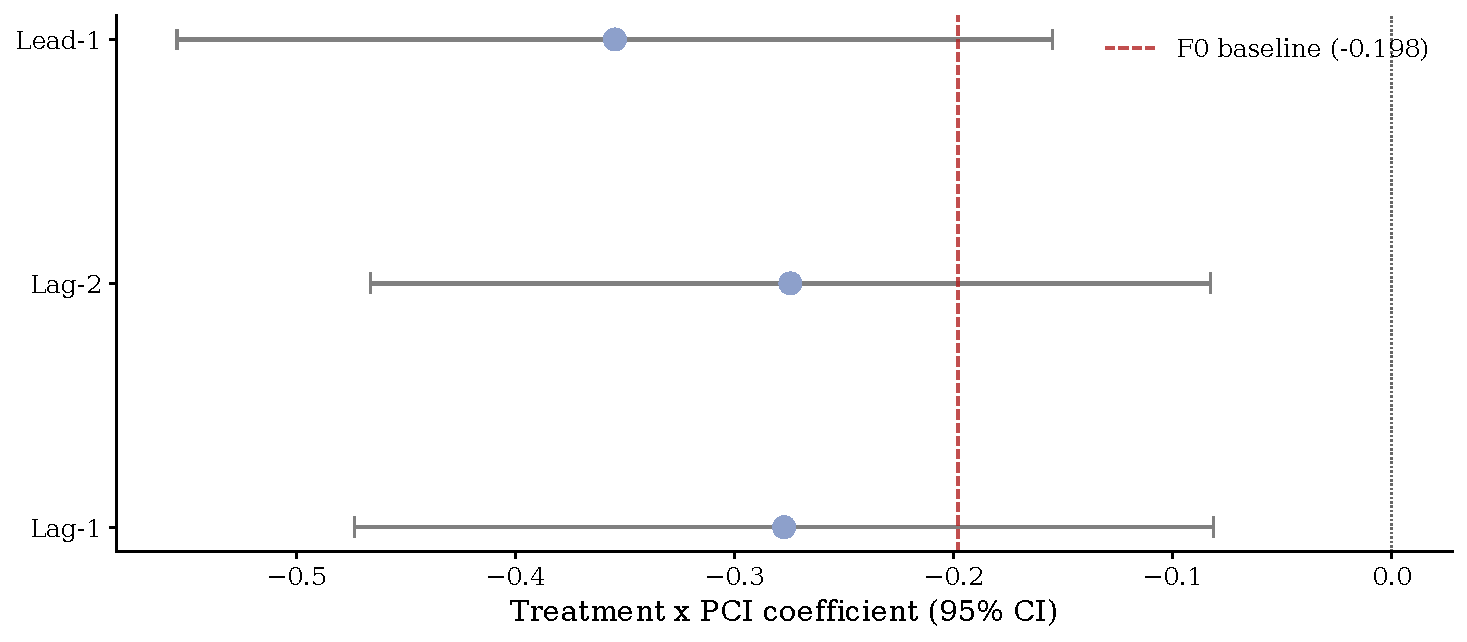
\includegraphics[width=0.8\textwidth]{figures/08_endogeneity/endogeneity_panel_checks.pdf}
\caption{Endogeneity Tests: Panel Specifications with Pair FE}
\label{fig:endo_panel}
\begin{minipage}{0.9\textwidth}
\footnotesize \textit{Notes.} Point estimates and 95\% confidence intervals from PPML on stratified subsample (2,000 treated + 1,000 control pairs). All specifications include exporter$\times$year, importer$\times$year, pair, and product FE. Clustered SE at pair level.
\end{minipage}
\end{figure}

\subsection*{A.2 Baseline vs. Lead Comparison}

Figure~\ref{fig:baseline_lead} compares the baseline de-risking coefficient with the forward-looking (lead) coefficient across years, visualizing the persistence pattern discussed in Section~\ref{sec:results}.

\begin{figure}[htbp]
\centering
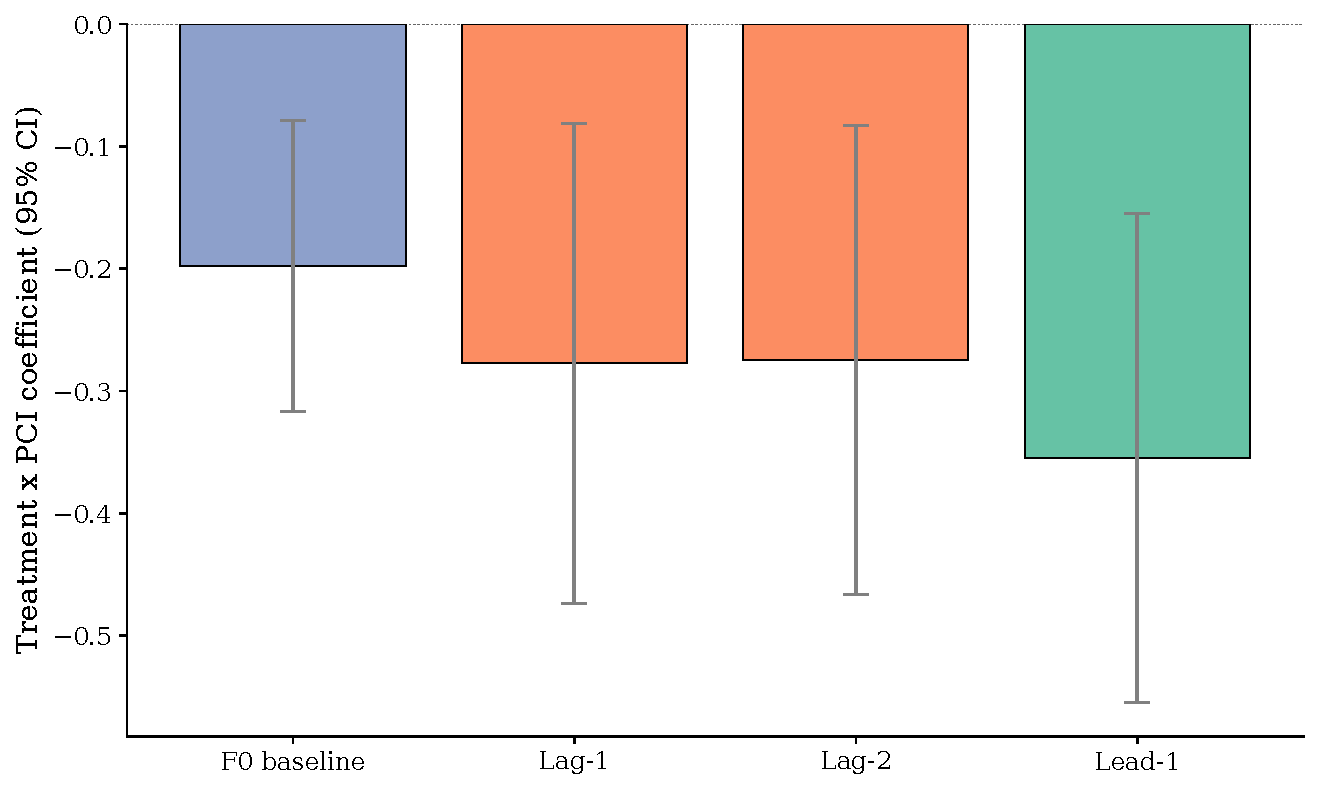
\includegraphics[width=0.7\textwidth]{figures/08_endogeneity/baseline_vs_lead.pdf}
\caption{Baseline vs. Lead De-risking Coefficients by Year}
\label{fig:baseline_lead}
\begin{minipage}{0.9\textwidth}
\footnotesize \textit{Notes.} Year-by-year PPML cross-sections. Baseline uses contemporaneous de-risking; Lead uses $t+1$ de-risking.
\end{minipage}
\end{figure}

\subsection*{A.3 Panel Robustness Specification Curve}

Figure~\ref{fig:spec_panel} presents the specification curve for panel pair-FE estimates across 11 robustness variants.

\begin{figure}[htbp]
\centering
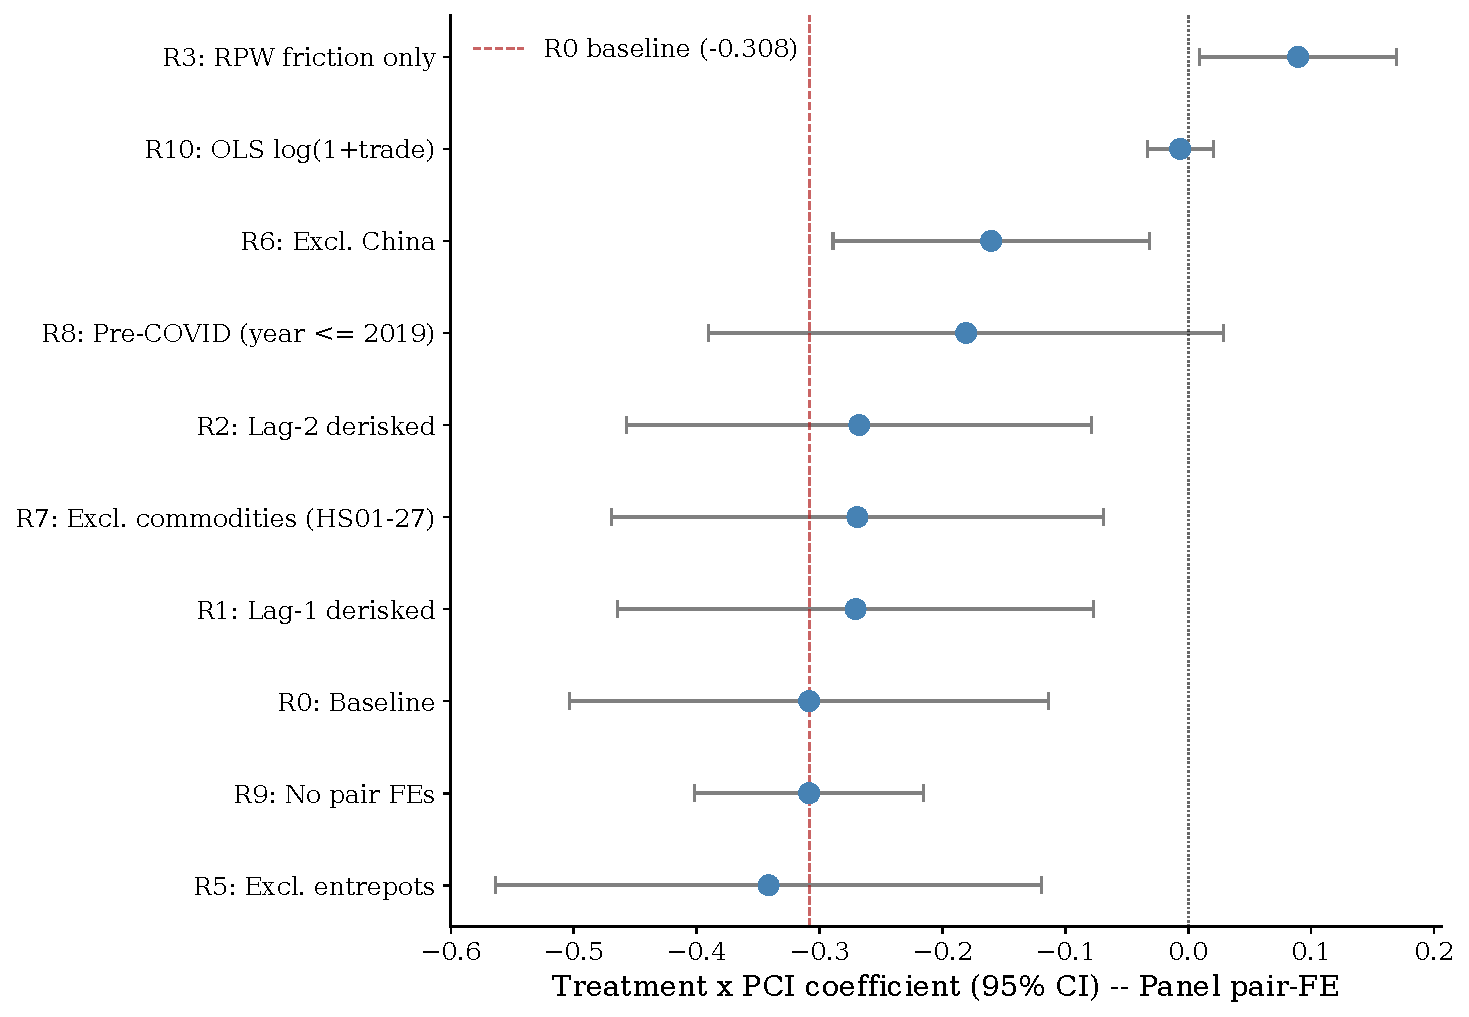
\includegraphics[width=0.85\textwidth]{figures/11_robustness/specification_curve_panel.pdf}
\caption{Specification Curve: Panel Robustness (Pair FE)}
\label{fig:spec_panel}
\begin{minipage}{0.9\textwidth}
\footnotesize \textit{Notes.} Each point represents one specification variant estimated with pair FE on the stratified subsample. Horizontal bars show 95\% confidence intervals.
\end{minipage}
\end{figure}

\subsection*{A.4 Falsification Test Results}

Figure~\ref{fig:falsification} presents the combined falsification panel, showing forest plots of yearly means and panel pair-FE results for all placebo interactions.

\begin{figure}[htbp]
\centering
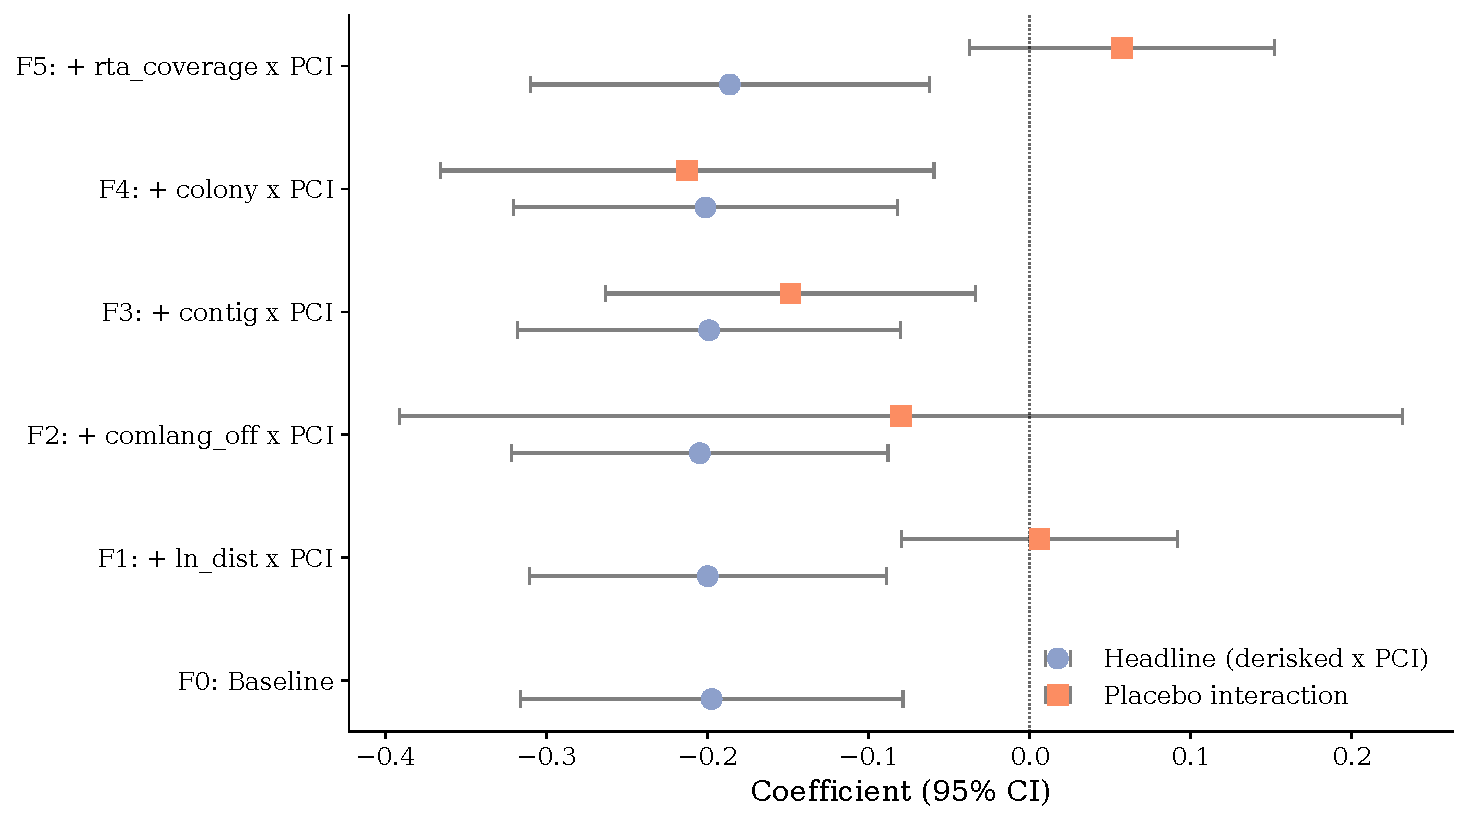
\includegraphics[width=0.85\textwidth]{figures/12_falsification/falsification_panel.pdf}
\caption{Falsification Tests: Forest Plot}
\label{fig:falsification}
\begin{minipage}{0.9\textwidth}
\footnotesize \textit{Notes.} Left panel: yearly mean coefficients with pooled 95\% CI. Right panel: permutation null distribution with baseline coefficient marked.
\end{minipage}
\end{figure}

\subsection*{A.5 De-risking Exposure World Map}

Figure~\ref{fig:derisking_map} maps the number of de-risked bilateral corridors per country.

\begin{figure}[htbp]
\centering
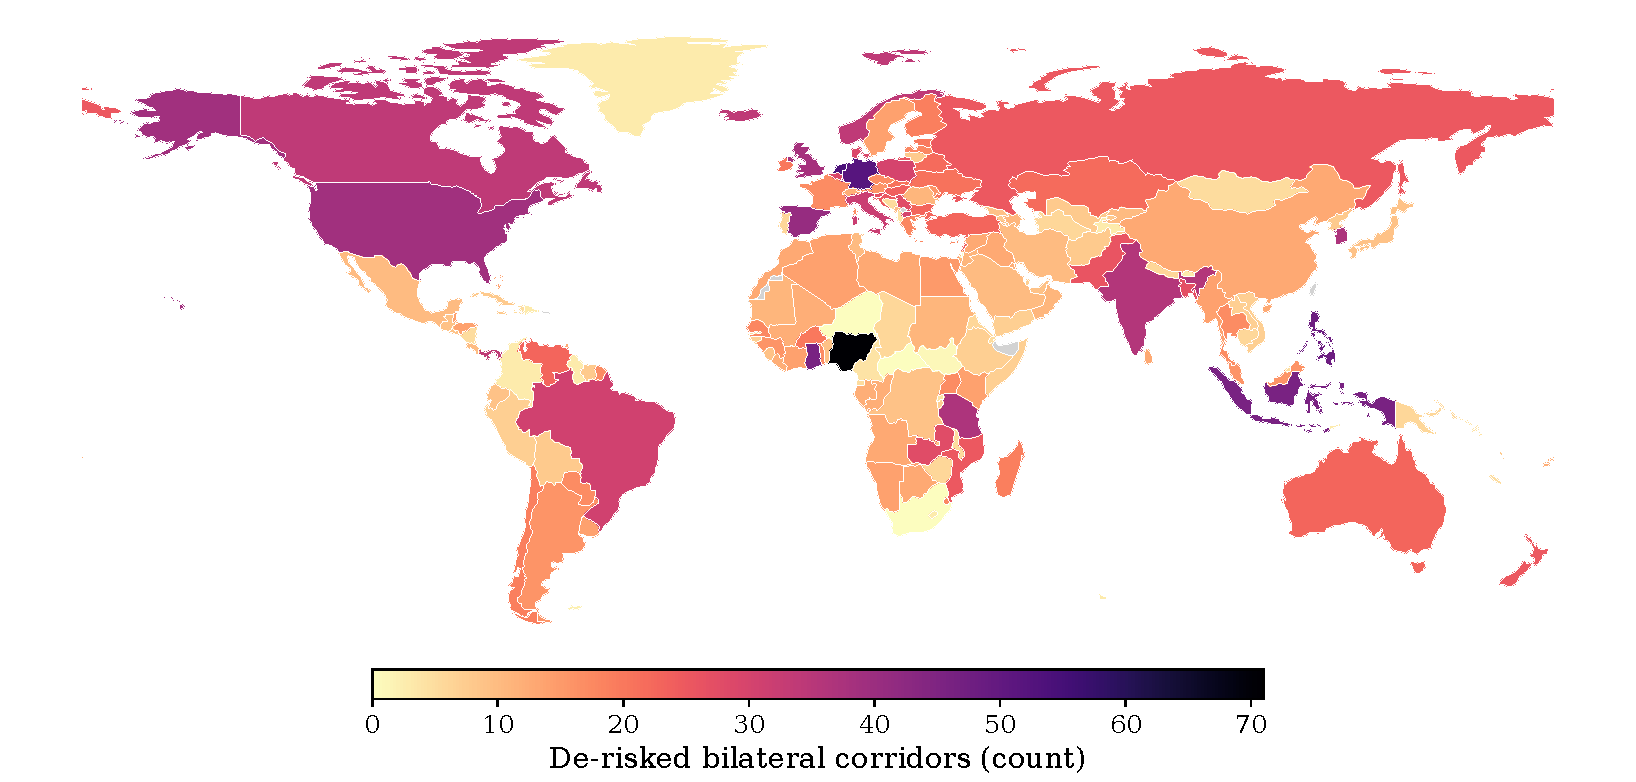
\includegraphics[width=0.95\textwidth]{figures/13_figures/world_derisking_exposure.pdf}
\caption{De-risking Exposure by Country}
\label{fig:derisking_map}
\begin{minipage}{0.9\textwidth}
\footnotesize \textit{Notes.} Country-level count of de-risked bilateral corridors (FDI dropped $>$50\% from the 2015--2017 base), plotted as a choropleth using Natural Earth low-resolution country polygons. Darker shading indicates more de-risked partners; countries with no data shown in light gray.
\end{minipage}
\end{figure}

\subsection*{A.6 SOS Decomposition}

Figure~\ref{fig:sos_decomp} decomposes the SOS into intensive and extensive margin contributions for the top 20 countries.

\begin{figure}[htbp]
\centering
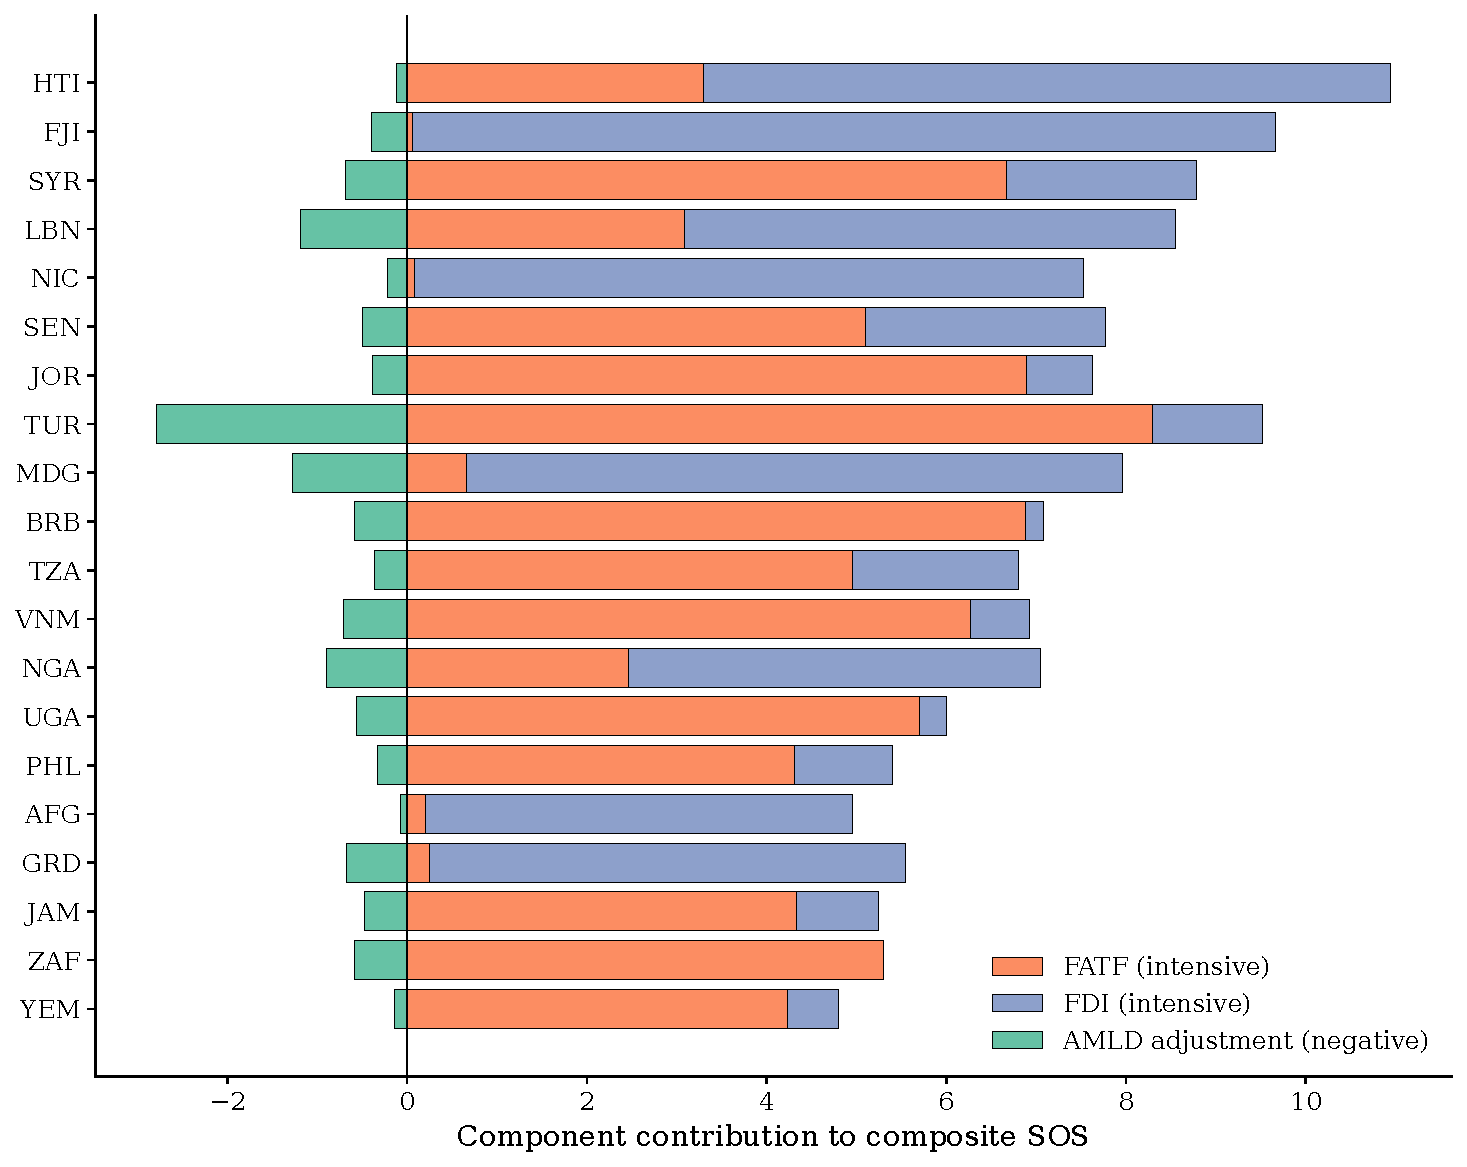
\includegraphics[width=0.8\textwidth]{figures/13_figures/sos_decomposition_top20.pdf}
\caption{SOS Decomposition: Intensive vs. Extensive Margin (Top 20)}
\label{fig:sos_decomp}
\begin{minipage}{0.9\textwidth}
\footnotesize \textit{Notes.} Stacked bar chart. Intensive margin: existing complex trade at risk in de-risked corridors. Extensive margin: unrealized diversification potential.
\end{minipage}
\end{figure}

\subsection*{A.7 SOS Validation: Conditional Scatter}

Figure~\ref{fig:validation} plots the SOS against the Chainalysis Global Crypto Adoption Index, both unconditionally and conditional on GDP per capita.

\begin{figure}[htbp]
\centering
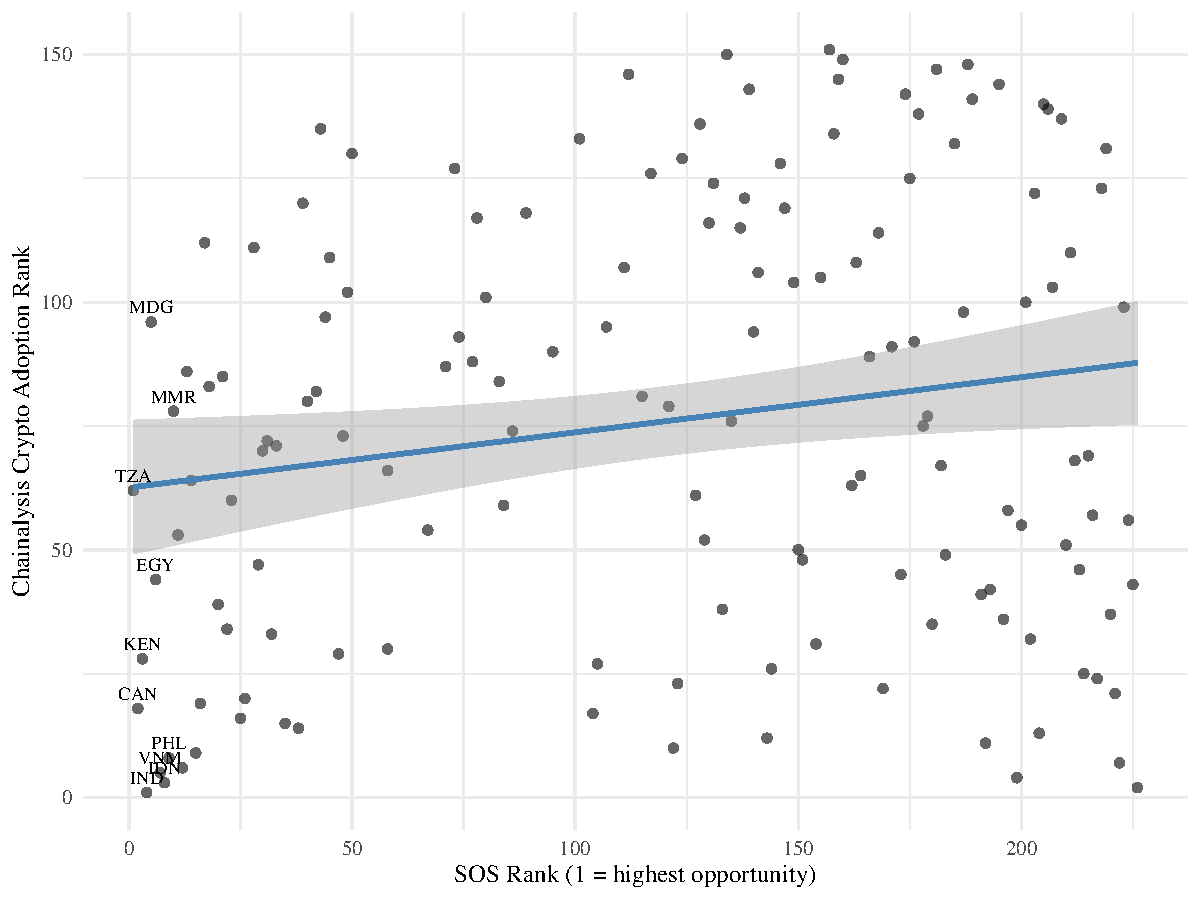
\includegraphics[width=0.7\textwidth]{figures/10_validation/sos_vs_chainalysis.pdf}
\caption{SOS vs. Chainalysis Crypto Adoption Index}
\label{fig:validation}
\begin{minipage}{0.9\textwidth}
\footnotesize \textit{Notes.} Each point is a country ($N = 149$). Unconditional Spearman $\rho = 0.155$; conditional on log GDP per capita, $\rho = 0.126$.
\end{minipage}
\end{figure}
